\titleformat{\subsection}{\large\bfseries\CJKsection}{\thesubsection}{1em}{}

\chapter{\term{HIP} 工具}
\label{chap:HIP Tools}

正如我們目前所看到,ROCm OS 提供的 HIP 支援,大幅簡化了平行 GPU 程式的開發。然而,要達到最佳效能,更深入了解最適合的方法是必須的。有些人也許會透過試錯法來調適出最佳效能,但使用效能分析工具可以提供系統化的方法,不僅幫助所有人節省時間與精力,還能最大限度地減少混亂。除此之外,針對不同的 GPU 架構開發或移植應用程式是個挑戰,尤其是移植 CUDA 應用程式到新的架構。在本章中,我們將探討 ROCm 提供的工具,這些工具可用於效能分析與移植應用程式到不同的 GPU 架構。

ROCm 提供程式設計者 \term{ROCmInfo},此命令列工具提供有關 ROCm 軟體堆疊(software stack)和系統硬體配置的詳細資訊。開發者可以在最佳化效能時,快速且簡單地取得系統設定的重要資訊。另外一個有用的工具是 ROCm System Management Interface (SMI,系統管理介面),可以幫助 GPU 程式設計者視覺化監控 GPU 的使用率、頻率、溫度等等的變數。根據 OS 的權限級別,程式設計者可以使用 ROCm SMI 調整 GPU 核心和記憶體頻率(在設備允許的範圍內)。為了定位及偵錯 kernel 的錯誤,ROCm 提供 rocgdb,這是一款基於 GNU 除錯器(GDB) 的工具,讓程式設計者逐步執行 kernel 原始碼。它可以檢查 wavefront 暫存器狀態。ROCm 也提供程式設計者 \term{rocProf},這是一款易使用的 GPU 硬體分析器,讓應用程式開發者了解應用程式在 GPU 的執行情況,並幫助識別潛在的效能瓶頸。ROCm 提供將 CUDA 程式碼庫轉換為 HIP 的工具。在許多情況下,程式設計者或研究人員需要在 AMD GPU 上執行 NVIDIA 系統的 CUDA 程式(例如:用來比較效能的差異)。在 HIP 出現之前,唯一的方法是手動將 CUDA 轉換成 OpenCL,一種繁瑣且容易出錯的路徑。\chapref{chap:Third-Party Tools} 也提供多種第三方工具的使用指南,這些工具可以用來分析 ROCm 所支援的 GPU 效能。

\section{\term{ROCmInfo}}

當談到最佳化程式碼以達到最大效能時,開發者通常依賴他們對所使用系統的理解。\term{ROCmInfo} 這款強大的命令列工具可以用來幫助獲得系統硬體及軟體的資訊。\term{ROCmInfo} 提供有關 ROCm 軟體堆疊(software stack)及系統硬體設定的詳細資訊。

有了\term{ROCmInfo},開發者可以輕鬆取得有關系統配置的關鍵資訊,從而更有效的優化他們的程式碼。這工具對開發 GPU 加速應用程式特別有幫助,因為它可以讓給開發者深入了解硬體的能力與限制。通常情況下,如果電腦上安裝了標準的 ROCm,則可以在 /opt/rocm/bin 目錄中找到 rocminfo。假設這個目錄在系統 PATH 變數中,開發者可以打開終端機(terminal)並輸入 \term{rocminfo},輕鬆取得有關 ROCm 堆疊(stack)及硬體的設定資訊。ROCm 本身建立在異質系統架構(HSA, the Heterogeneous System Architecture)之上,它定義了異質計算系統的標準化硬體架構和軟體介面。Rocminfo 當作是一個獲取有關系統 attributes 和 agents 資訊的入口,提供開發者綜合了解他們 HSA 標準的硬體設定。

在 ROCm 環境中,HSA 系統的 attributes 提供有價值的元資料(metadata),說明 GPU 及其相關系統資源的特性。透過使用「rocminfo」 工具,開發者可以查詢這些資訊,深入了解硬體性能,並進一步微調程式碼,以實現最佳化效能。HSA agents(HSA agent 是指可以執行 ROCm kernels 的設備)構成是系統的核心支柱,傳遞重要的系統資源,例如 CPUs 和 GPUs。在 ROCm 背景下,HSA agents 可以大致分成兩個種類:CPU agents 及 GPU agents。GPU agents 具體指的是支援 ROCm 的 AMD GPUs,其打開了 GPU 加速計算可能的世界。利用 rocminfo 提供有關 HSA agents 的知識,開發者可以充分發揮系統資源的潛力。這讓他們能夠設計及優化程式以充分利用 CPU 和 GPU 的功能,為應用程式帶來出色的效能提升。

\begin{figure}
    \centering
    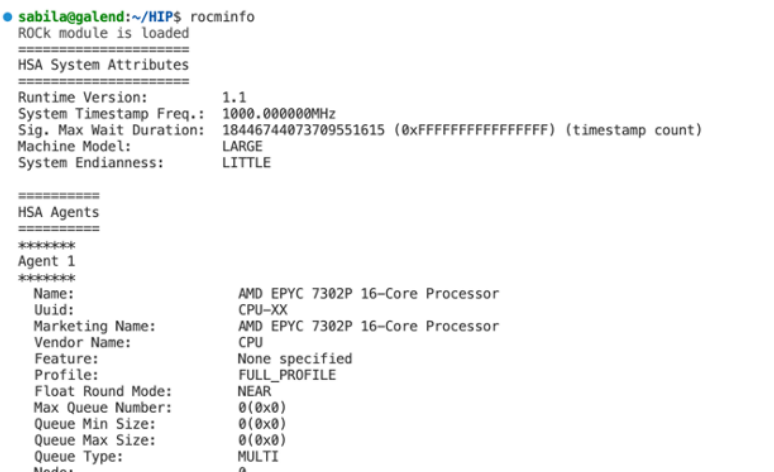
\includegraphics[width=0.75\linewidth]{FileAusiliari/Screenshots/Figure7-1.png}
    \caption{\bold{rocminfo}執行結果的截圖}
    \label{fig:rocminfo}
\end{figure}

如同我們稍早所講,rocminfo 是個可以讓開發者深入了解 GPUs 功能及配置的強大工具。\figref{fig:rocminfo} 展示了透過 rocminfo 獲得的一些寶貴資訊。這豐富的資訊提供開發者有關 GPUs 詳盡的細節,讓他們做出明智的決定、優化程式碼及微調應用程式,來利用 GPUs 的特定功能及能力。

在 ROCm 生態系統中,每個 HSA agent 會被指派一個獨一無二的識別符號,以便於計算任務的溝通及資源分配。這個識別符號是通用又唯一的識別碼,在系統中區分各個 agent。我們可以更仔細看 \figref{fig:HSA agent 1} 的範例螢幕截圖。在這範例中,我們觀察到 Agent 1 被識別為一個 16 個 kernel 的 CPU 設備。這些資訊讓開發者針對它們的程式碼,來去更有效的利用 Agent 1 的 CPU 資源、最佳化效能及有效執行任務。在 GPU 加速應用程式中,它能夠讓開發者對任務分配、資源利用和溝通策略做出明智的決定。

\begin{figure}
    \centering
    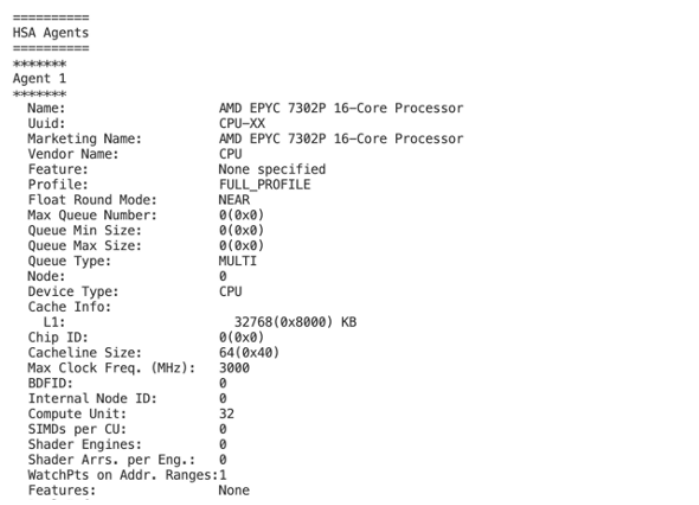
\includegraphics[width=0.75\linewidth]{FileAusiliari/Screenshots/Figure7-2.png}
    \caption{HSA agent 1 - 系統中的CPU}
    \label{fig:HSA agent 1}
\end{figure}

除了 Agent 1,我們還有 Agent 2 的寶貴資訊,如圖\figref{fig:HSA agent 2}。Agent 2 被識別為 Radeon Pro W6800 GPU 設備。這款 GPU 設備具備強大能力,可顯著提升計算效能。透過檢查 rocminfo 提供的資訊,我們發現 Radeon Pro W6800 GPU 包含三個級別的快取,即一個大小 16KB 的 L1 快取、一個大小 4MB 的 L2 快取及一個 大小 128MB 的 L3 快取。這些快取對於降低記憶體存取延遲及提升整體效能至關重要,因為它們能夠將頻繁訪問的資料儲存在更靠近CUs的位置。除此之外,Radeon Pro W6800 GPU 有 60 個 CUs ,使其成為強大的計算設備。每個計算單元內含 60 個 SIMD 單元。這種硬體架構設計使得 GPU 能夠在每個計算單元內,使用相同的指令,同時對不同的資料執行最多 60 個操作。這種平行化的能力顯著提升了高效計算密集型任務的能力。Radeon Pro W6800 GPU 的 wavefront 大小是 32,這表示每個 CU 可以平行化執行 32 個 threads。這種 threads 平行執行使 GPU 能夠同時處理多個 threads,提升吞吐量,並加速執行能夠平行化的工作負載。

了解 Radeon Pro W6800 GPU 的這些技術細節後,可以讓開發者深入了解這款高效能設備的底層架構和功能。開發者可以運用這些知識來最佳化他們的 GPU 加速應用程式,確保 GPU 資源充分利用,以達到最大效能。

\begin{figure}
    \centering
    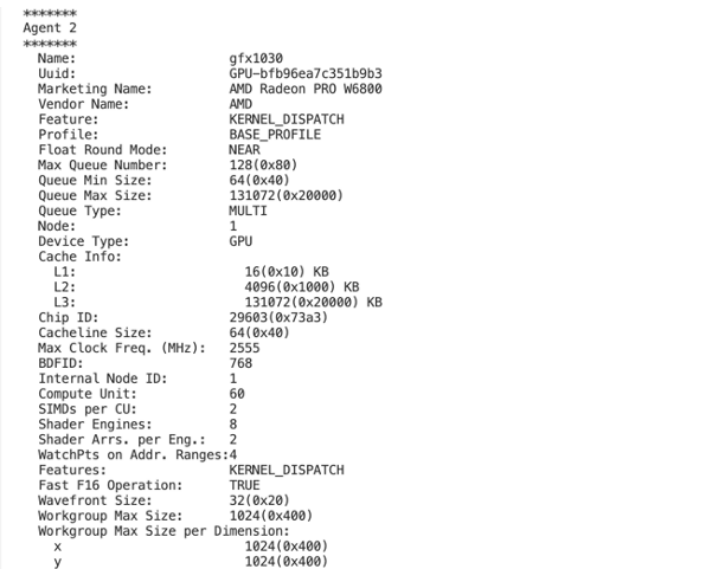
\includegraphics[width=0.75\linewidth]{FileAusiliari/Screenshots/Figure7-3.png}
    \caption{HSA agent 2 - 系統中的GPU}
    \label{fig:HSA agent 2}
\end{figure}

\section{\term{ROCm SMI}}

\term{ROCm SMI} 使系統管理員能夠追蹤多種系統階層的指標,例如電力、效能及溫度。通常情況下,如果電腦上安裝了標準的 ROCm,則可以在 /opt/rocm/bin 目錄中找到 \term{ROCm SMI}。假定這個目錄已經在 PATH 的環境變數中,開發者可以打開終端機並輸入 \term{rocm-smi},來存取和監控與 PCIe、電力管理、時脈、效能、錯誤及事件有關的各種系統層級參數。\term{ROCm SMI} 也可以提供一種簡便的方法,來檢查 \term{ROCm} kernel 驅動程式是否正確載入,並確保所有系統 GPUs 正確的初始化。

執行 \bold{rocm-smi -h} 可以查看 \term{ROCm SMI} 的版本所有可用的功能列表,其中 \bold{-h} 代表 「help (幫助)」。在本節中,我們將介紹這個工具的功能,並強調監控 GPU 資訊並不需要管理員權限。但若要改變時脈頻率和功率狀態則需要使用 \bold{sudo}。此外,可以執行 \bold{rocm-smi –showid}獲得 GPU ID,\bold{–showid} 讓使用者簡單地辨識和正在使用的 GPU 設備,這在多 GPU 系統特別有幫助,因為多 GPU 系統可能很難區分不同的設備。

除了提供 GPU 設備的資訊,\bold{ROCm SMI} 也允許使用者即時監控變動的硬體。透過使用 \bold{watch -n0 rocm-smi} 命令,可以取得 GPU 設備的溫度和平均消耗功率的即時更新。在這裡,\bold{watch} 是個標準的 Linux 命令,而 n0 代表盡可能最小執行 \bold{rocm-smi} 命令的間隔時間。這功能對於監控效能並及時發現運行過程中可能遇到的問題或異常,特別有幫助。

\term{ROCm SMI}通常用來看系統動態資訊,如圖 \figref{fig:Output of the ROCm SMI tool}。該輸出來自於本書開發期間的系統。擁有 8 張 GPUs(0-7),每個設備的 GPU 頻率設定為 800 MHz,而記憶體頻率設定為 1,600 Mhz。因為系統閒置,GPU 顯示隨機存取記憶體(VRAM)和使用率百分比都為 0\%。「perf」行顯示「auto」,代表動態功耗管理 (DPM) 的功能已經啟動,DPM 模組會根據系統的負載需求與功率限制,自動調整電壓與頻率。此外,可以用 \bold{rocm-smi} 改變 GPU 設定。我們注意到在\figref{fig:Output of the ROCm SMI tool}中,效能等級預設為auto(自動)。要修改這個,我們可以使用\bold{rocm-smi –setperflevel low} 命令去設定效能等級為低。透過這個調整,我們可以更有效地針對特定需求優化 GPU 效能,從而大幅提升工作負載的效率。

使用 \bold{rocm-smi –showsclkrange} 可以查詢 GPU 時脈頻率的列表,也可以使用 \bold{rocmsmi –showmclkrange} 查詢記憶體時脈頻率的列表。超級使用者權限的使用者可以調整時脈參數。舉例來說,\bold{–setclk} 用來調整圖形時脈,\bold{–setmclk} 用來調整記憶體時脈。不同 GPU 系統在調整時脈行為方面提供的彈性程度不同。因此,假如系統並不支援某些的設定,\term{ROCm SMI}會回傳\bold{NOT\_SUPPORTED}。

另一個有用的 \term{ROCm SMI} 命令是 \bold{–showtopo},呈現節點的拓譜圖。程式設計者可以在多 GPU 的系統上利用該資訊了解不同 GPUs 內部是如何連接的(例如:PCIe 或 AMD 的晶片間全域記憶體互聯)。該命令也會以 hops 表示 GPUs 間的距離,而 hops表示系統中從一個 GPU 到另一個 GPU 需經過的節點數。這在多 GPU 系統中可以用來優化溝通模式。

\begin{figure}
    \centering
    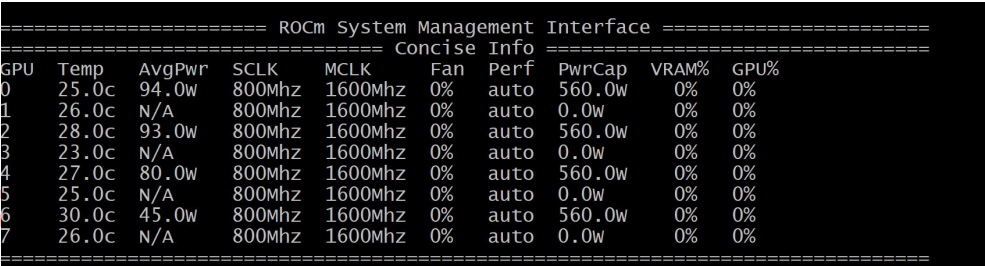
\includegraphics[width=0.75\linewidth]{FileAusiliari/Screenshots/Figure7-4.png}
    \caption{\term{ROCm SMI}工具的輸出}
    \label{fig:Output of the ROCm SMI tool}
\end{figure}

假如程式設計者想要在程式內調用 \term{ROCM SMI} 命令,而非透過 CLI,可以使用 \term{ROCm-SMI-Lib} 提供的 C/C++ 圖形化的使用者介面(GUI, graphical user interface),此開源的函式庫可以在Github \cite{amd2021rocm-smi-lib} 找到。目前支援的 APIs 集合寫在 rocm\_smi.h 標頭檔中。

\lstref{lst:ROCm-SMI-Lib} 給了一個可以存取 \term{ROCm SMI} 函式庫的程式範例。程式碼掃描使用者系統內的所有 AMD GPUs,並輸出每個 GPU 唯一的 PCI \bold{domain:bus:device:function} 辨識碼。此例行程序會初始化 \term{ROCm-SMI-Lib} 並檢測系統中 ROCm 設備的數量。接著,程式碼會逐一取回每個設備的 PCI 連接 \bold{domain:bus:device}。顯示完這些資訊後,程式呼叫 \term{rsmi\_shut\_down},執行程式結束前必要的清理。範例中有更多的細節,請參考函式庫的標頭檔 \term{rocm\_smi.h},它是開源儲存庫\cite{amd2021rocm-smi-lib}的一部分。

命令列工具和 API 層級呼叫都有它們的使用時機。假如在應用程式裡寫有關鎖定頻率、測量功率隨時間變化的程式碼,那麼 API 層級呼叫會非常有幫助。這通常用於擴展基準實驗,避免測量時需要查看 \term{ROCm SMI} 命令列工具的輸出。

\begin{lstlisting}[language=C, caption={\term{ROCm-SMI-Lib}範例}, label={lst:ROCm-SMI-Lib}]
#include <stdio.h>
#include <stdint.h>
#include "rocm_smi/rocm_smi.h"

int main() {
    rsmi_status_t ret;
    uint32_t num_devices;
    uint64_t bdf;

    // 為了清楚明瞭,跳過回傳程式碼檢查
    ret = rsmi_init(0);
    ret = rsmi_num_monitor_devices(&num_devices)

    for (int i=0; i < num_devices; ++i) {
        ret = rsmi_dev_pci_id_get(i, &bdf);
        printf("Device[%d] : PCI:%04lX:%02lX:%02LX:%02LX\n", i,
                        (bdf >> 32) & 0xffffffff, (bdf >> 8) & 0xff,
                        (bdf >> 3) & 0x1f, bdf & 0x7);
    }
    ret = rsmi_shut_down();
    return 0;
}
\end{lstlisting}

\section{\term{ROCm} 除錯器}
\label{sec:7.3}

設計良好的除錯器對於 GPU 程式設計者的支援至關重要。假如在應用程式執行時產生意外結果或崩壞,逐行執行 kernel 將有助於識別問題的根源。除錯器是檢測每個 thread 暫存器內容或檢視參數值的重要工具。為了這些目的,ROCm 提供 \term{rocgdb} 除錯器,它基於\term{GDB}之上建造,而\term{GDB}是一個用在CPU應用程式除錯的工具。

在本節中,我們將學習如何使用 \term{rocgdb} 有效地除錯並輸出 wavefront 的資訊。我們的範例中,每個 thread 會從輸入陣列讀取一個元素,將該元素乘以 thread ID,並將結果儲存在輸出陣列。輸入陣列的值會被初始化,使得第 i 個元素值為 i。採用這簡單的協定,索引 0 值為 0,索引 1 值為 1,以此類推。在一開始 kernel 執行時,我們計算 thread ID 來獲得輸入和輸出陣列的起始位置。在 \lstref{lst:Scalar multiply kernel} 的第18行,我們讀 \bold{a} 陣列和 thread ID。我們將它們相乘並把結果儲存在\bold{c}陣列中。我們的範例中,總共使用 256 threads,每個 workgroup 大小為 64。因此,總共有 4 個 workgroups,每個 workgroups 有 64 個threads。

我們的範例在每個 wavefront 有 64 個 threads 的 AMD GPU 上編譯並執行。請記住,系統總共有 4 個 wavefronts,並注意先前介紹的 thread 概念和「\term {GDB} threads」的不同。\term{GDB} threads 可能指在執行期間 OS 產生的 host-side thread,或是專門對應於 \term{GDB} thread 的 wavefront。因此,如果我們僅關注 device-side \term{GDB} threads,而我們的範例執行包含四個 wavefronts,因此總共有四個 device-side \term{GDB} threads。在下面的例子中,當提及「threads」和「thread IDs」時,才代表實際執行在 GPU 的 threads。只有明確提及「debugger」 threads 才是「GDB」 threads。

為了檢查 wavefront 0 的暫存器值,我們按照以下步驟:

\begin{enumerate}
    \item 任何 GPU kernel 除錯之前,我們必須使用 \bold{-g} 編譯選項來編譯程式,這樣除錯資訊就會包含在輸出的二進位檔中。如同範例,我們執行 \bold{hipcc -g scale\_hip.cpp -o scale\_hip},可以產生檔名為 \term{scale\_hip} 的二進位檔。
    \item 現在,我們準備用\term{rocgdb} 進行除錯。為了啟動除錯階段,我們輸入 \bold{rocgdb ./scale\_hip}。進入除錯環境後,我們從\term{GDB}環境的 CLI 執行目標程式。
    \item 我們在 kernel 的第 19 行設定斷點,這行是計算完後,輸出結果的地方。要使用\term{GDB} CLI 中設定斷點,我們輸入\bold{break scale\_hip.cpp:19}。接著,我們繼續使用\term{GDB}命令執行,\bold{c}(即 continue 命令)。由於所有 wavefronts 都遵循相同的控制流,因此每個 wavefront 都會命中(hit)該斷點。
    \item 設定多個斷點後,我們可以分析每個斷點的程式狀態,並深入了解其邏輯。當斷點設定完成後,我們可以在 GDB 的命令列使用 \bold{info b} 命令,查看我們在程式中設定的斷點狀態和詳細資訊。此詳細資訊包含設定了多少斷點、提供每個設定斷點的程式碼行數以及斷點 ID (為一個數字)。
    \item 我們可以使用\bold{r}(run,執行)命令開始除錯。此命令會啟動程式,依照設定的斷點執行,並在第一次遇到斷點時暫停執行。
    \item 在到達斷點後,\bold{c}(continue,繼續)命令使我們能夠從當前的斷點重新執行程式。使用這命令後,除錯器會繼續執行程式,直到碰到下一個斷點,在那時再次暫停程式執行。此功能有助於透過更大步數執行程式碼,來分析程式在不同階段的行為。
    \item 接著,我們使用 \bold{info threads} 查看當前活動的 threads 列表。輸出結果如同在 \lstref{lst:Output of info threads command}。我們在這討論的是 \term{GDB} threads,不要將其與在 GPU 上執行的 threads 混淆。\term{GDB} threads IDs 1、2和3是作業系統產生的 host-side threads。Thread IDs 5、6、7和8指的是 kernel 啟動的四個 wavefronts。\term{GDB} Thread 5 旁的星號表示 wavefront 已到達斷點。
    \item 接下來,我們檢查當前在斷點執行的程式碼。假如我們在CPU進行除錯,可能會使用「l」或「list」命令來檢查程式碼。在GPU程式也相同。然而,由於 GPU 的二進位檔經過最佳化,可能很難確定組合程式碼執行的位置,或變數如何對應到暫存器。因此,GPU 除錯一般是在組合語言層級進行。假如讀者不熟悉 AMD GPU 的組合語言,請參考 \chapref{chap:AMD_GPU_internal} 中的詳細介紹。我們可以使用 \bold{disassemble} 命令來檢查組合語言程式碼,使用該命令後,會顯示一系列的組合語言程式碼,每條指令都有對應的記憶體位址。
    \item 為了檢查這個 wavefront 的暫存器的值,我們可以輸入\term{GDB}命令,\bold{info registers},它會輸出所有與當前作用中 thread 相關的暫存器資訊:thread ID 為 5,隸屬於 wavefront 0。\lstref{lst:Partial output of info registers command} 則顯示了該命令的部分輸出結果。有了這些資訊,程式設計者可以透過查看組合語言層級的 kernel 程式碼,來確認輸出值儲存在哪個特定的暫存器。在 \bold{GDB} 除錯階段中,可以使用 \bold{disassemble scaleKernel} 命令輕鬆的達到。

    繼續看我們的範例,我們觀察到暫存器 v3 將值寫回至主記憶體前,儲存了最終結果。因此,透過檢查\lstref{lst:Partial output of info registers command}的第 4 行,我們可以查看 wavefront 0 中所有64個 threads 的暫存器 v3 的值。舉例來說,第三個數值為 0x4,對應於該 wavefront 的 thread ID 2。具體而言,thread ID 2 會從輸入陣列 \bold{a} 中讀取數值 2,將其與自身的 thread ID(值為2)相乘,最終輸出 0x4。

    \item 程式繼續執行後,不同的 wavefront 會再次命中(hit)該斷點。我們可以接著檢查該 wavefront 的其他暫存器值。

\end{enumerate}

\begin{lstlisting}[language=C, caption={純量乘法kernel}, label={lst:Scalar multiply kernel}]
#include "hip/hip_runtime.h"
#include <stdio.h>
#include <stdlib.h>
#include <math.h>
#define HIP_ASSERT(x) (asert((x)==hipSuccess))

// HIP kernel. 每個 thread 負責 c 的一個元素
__global__ void scaleKernel(int *a,int *c, int n)
{
    // 取得我們的全域 thread ID
    int id = blockIdx.x*blockDim.x+threadIdx.x;
    // 確認我們沒有超出邊界
    if (id < n)
    {
    
        c[id] = id*a[id];
    }
}
\end{lstlisting}

\begin{lstlisting}[language=bash, caption={info threads命令的輸出結果}, label={lst:Output of info threads command}]
Id Target Id Frame
1 Thread 0x7ffff7fdc880 (LWP 58984) "a.out" 0x00007ffff5fc9ef7 in sched_yield () from /lib/x86_64-linux-gnu/libc.so.6
2 Thread 0x7ffff4f9e700 (LWP 58990) "a.out" 0x00007ffff5fdc317 in ioctl () from /lib/x86_64-linux-gnu/libc.so.6
4 Thread 0x7ffff4573700 (LWP 58992) "a.out" 0x00007ffff5fdc317 in ioctl () from /lib/x86_64-linux-gnu/libc.so.6
* 5 AMDGPU Thread 2:1:1:1 (0,0,0)/0 "a.out" scaleKernel (a=<optimized out>, c=<optimized out>, n=<optimized out>) at vadd_hip.cpp:20
6 AMDGPU Thread 2:1:1:2 (1,0,0)/0 "a.out" scaleKernel (a=<optimized out>, c=<optimized out>, n=<optimized out>) at vadd_hip.cpp:20
7 AMDGPU Thread 2:1:1:3 (2,0,0)/0 "a.out" scaleKernel (a=<optimized out>, c=<optimized out>, n=<optimized out>) at vadd_hip.cpp:20
8 AMDGPU Thread 2:1:1:4 (3,0,0)/0 "a.out" scaleKernel (a=<optimized out>, c=<optimized out>, n=<optimized out>) at vadd_hip.cpp:20
\end{lstlisting}

\begin{lstlisting}[language=bash, caption={info registers 命令的部分輸出結果}, label={lst:Partial output of info registers command}]
v0          {0xe8202000, 0xe8202004, 0xe8202008, 0xe820200c, 0xe8202010, 0xe8202014, 0xe8202018, 0xe820201c, 0xe8202020, 0xe8202024, 0xe8202028, 0xe820202c, 0xe8202030, 0xe8202034, 0xe8202038, 0xe820203c, 0xe8202040, 0xe8202044, 0xe8202048, 0xe820204c, 0xe8202050, 0xe8202054, 0xe8202058, 0xe820205c, 0xe8202060, 0xe8202064, 0xe8202068, 0xe820206c, 0xe8202070, 0xe8202074, 0xe8202078, 0xe820207c, 0xe8202080, 0xe8202084, 0xe8202088, 0xe820208c, 0xe8202090, 0xe8202094, 0xe8202098, 0xe820209c, 0xe82020a0, 0xe82020a4, 0xe82020a8, 0xe82020ac, 0xe82020b0, 0xe82020b4, 0xe82020b8, 0xe82020bc, 0xe82020c0, 0xe82020c4, 0xe82020c8, 0xe82020cc, 0xe82020d0, 0xe82020d4, 0xe82020d8, 0xe82020dc, 0xe82020e0, 0xe82020e4, 0xe82020e8, 0xe82020ec, 0xe82020f0, 0xe82020f4, 0xe82020f8, 0xe82020fc}
v1          {0x7fff <repeats 64 times>}
v2          {0x0 <repeats 64 times>}
v3          {0x0, 0x1, 0x4, 0x9, 0x10, 0x19, 0x24, 0x31, 0x40, 0x51, 0x64, 0x79, 0x90, 0xa9, 0xc4, 0xe1, 0x100, 0x121, 0x144, 0x169, 0x190, 0x1b9, 0x1e4, 0x211, 0x240, 0x271, 0x2a4, 0x2d9, 0x310, 0x349, 0x384, 0x3c1, 0x400, 0x441, 0x484, 0x4c9, 0x510, 0x559, 0x5a4, 0x5f1, 0x640, 0x691, 0x6e4, 0x739, 0x790, 0x7e9, 0x844, 0x8a1, 0x900, 0x961, 0x9c4, 0xa29, 0xa90, 0xaf9, 0xb64, 0xbd1, 0xc40, 0xcb1, 0xd24, 0xd99, 0xe10, 0xe89, 0xf04, 0xf81}
v4          {0x7fff <repeats 64 times>}
v5          {0x7fff <repeats 64 times>}
\end{lstlisting}

如同我們所看到,\term{rocgdb} 讓我們能夠透過設定斷點除錯 GPU kernels,並且逐個斷點跳轉。我們還可以在每個斷點取得詳細的執行資訊,包含在 wavefront 裡暫存器的細節。

\section{\term{ROCm} 分析器}

當談到最佳化 GPU 效能時,分析和追蹤是兩個必要的工具,可以幫助開發人員深入了解他們的應用程式是如何利用 GPU 設備。ROCm 提供兩個強大的工具幫助分析及追蹤:\term{ROCTracer} 和 \term{rocprofiler}。

\subsection{ROCTracer}

\term{ROCTracer} 用於評估應用程式的效能,在 GPU 分析模式下,它可以提供來自 GPU 硬體效能計數器的更詳細測量數據。\term{ROCTracer} 透過追蹤應用程式的執行過程,測量每個函式或程式碼區塊的執行時間,以評估應用程式效能。\term{ROCTracer} 能幫助開發人員識別出最耗時的程式碼區塊,並讓程式設計師專注於最佳化這些區塊。進行應用程式追蹤時,我們有多種選項可以使用。系統架構分為三個層級:底層為硬體、中間層為作業系統(例如 AMD KFD 驅動程式)、頂層則包括應用介面(例如 HSA 和 HIP 的執行)。我們可以在不同層級執行應用程式追蹤。舉例來說,若我們使用\bold{–hip-trace}選項,系統將會在使用者層級追蹤 HIP 執行時的位置,而使用\bold{–hsa-trace}選項則會啟動 HSA 層級的追蹤,至於使用\bold{–kfd-trace}選項,則可用來追蹤 AMD KFD 驅動程式的執行狀況。通常,在較高層級進行追蹤,有助於使用者將追蹤結果對應到原始碼,從而更快知道問題的根源。而透過較低階層的追蹤,則能獲得更詳細的效能分析資訊。

要用\term{ROCTracer}執行應用程式追蹤,我們可以根據我們追蹤的應用程式(為二進位檔),使用\bold{rocprof –hiptrace <your\_application>}命令。使用這個命令後,程式設計者將產生 4 個輸出檔案,其中包含應用程式執行時的相關資訊。檔案\term{results.copy\_stats.csv}(\lstref{lst:results.copy_stats.csv output})記錄每次 hip 執行時函式呼叫的時間資料,並以 CSV 格式呈現。該檔案包含執行時記憶體在 device 與 host 間複製所花費的時間,資料以奈秒為單位表示。

\begin{lstlisting}[language=bash, caption={\term{results.copy\_stats.csv} 在應用程式追蹤模式下的輸出結果}, label={lst:results.copy_stats.csv output}]
"Name","Calls","TotalDurationNs","AverageNs","Percentage"
"CopyDeviceToHost",2,9654400,4827200,81.6235566612597
"CopyHostToDevice",2,2173558,1086779,18.376443338740298
\end{lstlisting}

檔案\term{results.hip\_stats.csv}(\lstref{results.hip_stats.csv output})匯總了執行時間,並依 API 細分。除了先前介紹過的 APIs,該檔案也包含三個 APIs 的執行時間,分別為 \term{hipLaunchKernel}、\term{\_\_hipPushCallConfiguration} 及 \term{\_\_hipPopCallConfiguration}。這三個函式是實際的 API 呼叫,它們與 kernel 啟動時所使用的三角括號語法(Triple angle bracket syntax, \code{<<< >>>}) 有關。當 kernel 啟動時,HIP 會透過 \_\_hipPushCallConfiguration API ,將呼叫配置傳送給 GPU,這些配置包含 kernel 的維度、流(stream)、本地記憶體大小和 kernel 參數。接著,\term{hipLaunchKernel} 命令會啟動 kernel 的執行。最後,\term{\_\_hipPopCallConfiguration} 負責清除 kernel 的相關資訊,讓下個 kernel 執行時不受影響。

\begin{lstlisting}[language=bash, caption={\term{results.hip\_stats.csv} 在應用程式追蹤模式下的輸出結果}, label={results.hip_stats.csv output}]
"Name","Calls","TotalDurationNs","AverageNs","Percentage"
"hipMemcpy",4,537814533,134453633,99.25629643299268
"hipDeviceSynchronize",1,2834079,2834079,0.5230431088750803
"hipLaunchKernel",1,766035,766035,0.141375497262822228
"hipMalloc",3,246963,82321,0.04557822675271806
"hipFree",3,125437,41812,0.02315001044359153
"hipEventRecord",2,34503,17251,0.00636769701392124
"hipEventElapsedTime",1,6146,6146,0.0011342742905706734
"__hipPushCallConfiguration",1,5727,5727,0.0010569457959808406
"hipEventCreate",2,5238,2619,0.0009666984598127542
"hipEventSynchronize",1,2794,2794,0.0005156463338520113
"__hipPopCallConfiguration",1,2793,2793,0.0005154617789723219
\end{lstlisting}

還有另一個輸出檔案是\term{results.stats.csv}(\lstref{lst:results.stats.csv output})。該檔案匯總了 kernel 的執行時間。最後,除了匯總的資料之外,我們還想要一個更詳細的資料版本。在這種情況下,可以使用 \term{results.json} 檔案。雖然此檔案對人來說是可讀的,但仍需要花費精力,因此可以透過視覺化來更輕鬆地追蹤與了解執行的過程。檔案\term{results.json}根據標準追蹤格式,使我們能夠使用 chrome 追蹤工具來視覺化執行追蹤。我們首先在 Chrome 瀏覽器中輸入 \url{chrome://tracing},接著將我們的 json 檔上傳至該頁面。我們就可以視覺化追蹤該內容了。

\begin{lstlisting}[language=bash, caption={\term{results.stats.csv} 在應用程式追蹤模式下的輸出結果}, label={lst:results.stats.csv output}]
"Name","Calls","TotalDurationNs","AverageNs","Percentage"
"vector_add(float*, float*, float*, int)",1,2850719,2850719,100.0
\end{lstlisting}

\subsection{rocprofiler}

如同先前所提,在 kernel 執行時,\term{rocprof} 允許程式設計者取得硬體計數器的分析資訊。此計數器的值可以幫助程式設計者更好地了解,要如何在各種基於軟體的優化上提升硬體使用率。\term{rocprof} 可以產生快取命中(hits)和未命中(misses)的統計資料、不同類型指令的執行頻率、等待記憶體指令完成所花費的時間和其他與效能相關的關鍵資訊。分析器還可以針對群體裡的 kernels 進行選擇性的分析規則,或甚至只針對特定的 kernel。

請注意,GPU 硬體計數器的數字與 GPU 架構上的數字不同。嘗試優化應用程式效能的第一步是使用\bold{rocprof –list-basic}取得 GPU 硬體計數器的詳細資訊。輸出會包含基本硬體計數器的列表。除此之外,\bold{rocProf –list-derived} 可以看到分析器所產生的指標,這些指標由基本硬體計數器收集。程式設計者可以選擇特定的資料集去量化分析所帶來的開銷。這一點非常關鍵,因為每個 GPU 擁有的計數器數量是有限的,且只能收集這些計數器的資料。當程式設計者指定大量效能計數器進行分析時,硬體會重複執行 GPU kernels 去收集資訊,最終導致分析時間增加。\term{rocProf} 有支援兩種模式:i)效能分析,用於測量kernel執行時間,以及 ii)效能計數器,用於收集指定硬體計數器的資料。

接著,我們考慮在 \chapref{chap:getting_started_with_hip_programming} 的 \term{vector\_add} kernel 分析範例。我們使用\term{hipcc}編譯我們的應用程式,產生輸出二進位檔,\term{vadd}。因為我們想要收集 kernel 的執行時間,因此先使用效能分析模式。透過使用 \bold{rocprof –stats <your\_application>} 命令完成,它的輸出檔為\term{results.stats.csv},如圖\lstref{lst:rocProf output} 所示。這
逗號分隔值(CSV)檔案裡有統計資料,像是 kernel 被呼叫的次數(其中一個在我們的範例)、kernel 執行時的總時長與平均時長(5,920 ns 為 vadd),以奈秒為單位,以及 kernel 執行時佔 GPU 應用程式全部時間的比例(因為只有一個 kernel,因此我們的範例為100\%)。這些效能分析測量有助於找出應用程式中有哪些活動的 kernels,並提供每個 kernel 執行時的分類。這些資訊將協助程式設計者,使他們能夠減少消耗大部分時間的 kernels 集合。

\begin{lstlisting}[language=bash, caption={\term{rocProf} 在效能測量模式下的輸出結果}, label={lst:rocProf output}]
"Name","Calls","TotalDurationNs","AverageNs","Percentage"
"vecAdd(double*, double*, double*, int) [clone.kd]",1,5920,5920,100.0
\end{lstlisting}

然後,我們透過使用效能計數器模式的範例,說明如何收集硬體效能計數器的資訊。\lstref{lst:rocProf input file}顯示範例輸入檔,\term{input.txt}。第一行為「pmc」,指定我們分析執行時希望收集的計數器。在這範例中,我們收集\bold{TCC\_EA\_RDREQ\_sum}和\bold{TCC\_EA\_WRRREQ\_sum}。這些計數器分別統計快取與主記憶體發生讀取與寫入的次數。第二行指定我們希望分析的呼叫範圍。在這個案例中,我們只有一個呼叫;因此,我們指定0:1。如果在應用程式中多次啟動該 kernel,我們可以相對應地指定我們想分析的特定執行。舉例來說,如果我們想要分析 100 次中的第 55 次呼叫,我們只需指定「55」。如果從第 55 次開始分析接下來的所有呼叫,我們設定範圍為「55:」。第三行為「gpu」,指定我們希望分析的 GPU ID。在多 GPU 系統中,此數字可以針對所討論的 GPU 相對應的設定。最後一行是「kernel」行,指定 kernel 名稱。要分析多個 kernels,我們使用逗號分隔符。而這範例我們只解決了單一 kernel,\term{vecAdd}。我們有了輸入檔後,就準備好對\term{vector\_add} kernel 進行分析了。要分析它的執行,我們用\bold{rocprof -i input.txt -o vadd\_profile.csv ./vadd} 傳遞輸入文字檔給分析器,觸發 \term{rocProf} 分析所需的指標。最後的輸出結果儲存在 \term{vadd\_profile.csv},如圖 \lstref{lst:rocProf output file for the vectorAdd kernel} 所示。回想一下,這個名稱是我們使用 \bold{-o} 傳遞給 \term{rocprof} 的參數。輸出檔包含許多不同的值,像是 kernel 的名稱、process ID 和暫存器的使用情況。在文件尾端,我們可以看到兩個分析指標:\bold{TCC\_EA\_RDREQ\_sum} 和 \bold{TCC\_EA\_WRREQ\_sum}。它們輸出分別為「2610」和「1280」,因為該 kernel 讀取次數是寫入次數的兩倍(即 \term{vadd} 讀取 \bold{a} 和 \bold{b} 與寫入 \bold{c})。

\begin{lstlisting}[language=bash, caption={用於 vectorAddkernel 的\term{rocProf} 輸入檔}, label={lst:rocProf input file}]
pmc: TCC_EA_RDREQ_sum, TCC_EA_WRREQ_sum
range: 0:1
gpu: 0
kernel: vecAdd
\end{lstlisting}

\begin{lstlisting}[language=bash, caption={用於 vectorAddkernel的\term{rocProf}輸出檔}, label={lst:rocProf output file for the vectorAdd kernel}]
Index,KernelName,gpu-id,queue-id,queue-index,pid,tid,grd,wgr,lds,scr,vgpr
,sgpr,fbar,sig,obj,TCC_EA_RDREQ_sum,TCC_EA_WRREQ_sum
0,"vecAdd(double*, double*, double*, int) [clone .kd]"
,0,0,0,15239,15242,10240,256,0,0,12,24,0,0x0,0x7f9ba4c45800,2610,1280
\end{lstlisting}

現在,我們已經學會如何使用 \term{rocprof} 分析器,在下一章中,我們將分析及優化整個 GPU 應用程式。分析器的目標是提供程式設計者有用的資訊,使其能夠針對性的優化。

\section{\term{ROCm} 分析器 V2}

ROCm 分析器的第二個版本隨 ROCm 6.0 推出,是 \bold{rocprof} 的非向後相容更新。由於與早期版本不相容,兩個版本可以在標準的 ROCm 安裝下共同存在:\bold{rocprof} v1 和它的接替者。與 rocprof v1 類似,rocprof v2 也支援應用程式追蹤和 kernel 分析模型。

\subsection{應用程式追蹤}

使用 rocprofv2 和各種追蹤選項來追蹤 HIP/HSA API、非同步化的活動和 kernel 的調度。這些追蹤選項將顯示如下。請注意,這些命令尚未產生輸出,我們需要輸入外掛程式(即將會介紹)去產生輸出。

\begin{lstlisting}[language=bash, caption={使用rocprofv2應用程式追蹤功能的命令}, label={lst:trace feature of rocprofv2}]
# HIP API & 非同步活動追蹤
rocprofv2 –hip-api <app_relative_path>
rocprofv2 –hip-activity <app_relative_path>

# HIP API & 非同步活動追蹤
rocprofv2 –hsa-api <app_relative_path>
rocprofv2 –hsa-activity <app_relative_path>

# Kernel 調度追蹤
rocprofv2 –kernel-trace <app_relative_path>

# HIP & HSA API 與非同步活動追蹤與 Kernel 調度追蹤
rocprofv2 –sys-trace <app_relative_path>
\end{lstlisting}

rocprofv2 命令列支援在 HIP 和 HSA 兩種層級的 APIs 追蹤。通常來說,HIP APIs 可以直接與使用者程式進行互動,使用者可以將追蹤結果直接對應到程式,這樣分析 HIP 追蹤會更加簡單。HSA API 追蹤更加適合想要了解更低層級硬體行為的進階用戶。

HIP 和 HSA APIs 都支援非同步行為(即非同步記憶體複製)。如果選擇 –hip-api 或 –hsa-api,追蹤將只會紀錄 API 的執行時間,但不包含相關動作(例如:記憶體複製)所需的時間。要記錄真實動作的時間,可以使用 –hipactivity 和 –hsa-activity 選項。除此之外,為了記錄 kernel 執行,rocprofv2 命令列提供專門的 –kernel-trace 選項。

一個分析執行裡,可以有很多個追蹤選項同時使用。使用者可以用 –sys-trace 命令來簡化命令,而它包含上述提及的所有追蹤。

rocprofv2 命令列使用模組化的外掛程式系統來讓使用者選擇分析的輸出格式。ROCProfilerV2 附隨的外掛程式和輸出格式的描述列在 Table \ref{tab:plugins}。

\begin{table}[htbp]
    \centering
    \begin{tabular}{p{4cm}p{10cm}}
        \toprule
        \multicolumn{1}{c}{外掛程式} &
        \multicolumn{1}{c}{輸出格式} \\
        \midrule
        File & 文字檔 (.txt) \\
        Perfetto & Protobuf,採用 Chromium 專案追蹤事件格式 \\
        Advanced Thread Tracer &  二進位檔,用於視覺化分析工具 \\
        CTF & 二進位檔,採用CTF格式,能夠被 Babeltrace 等公共工具處理 \\
        OTF2 & 二進位檔,採用開放式追蹤格式版本2(OTF2),此追蹤可以被 Score-P、TAU 和 Vampire 等工具使用。 \\
        \bottomrule
    \end{tabular}
    \caption{rocprofv2 支援的外掛程式}
    \label{tab:plugins}
\end{table}

要產生輸出,變數 \bold{OUTPUT\_PATH} 要設成目標的目錄,否則不會產生輸出。唯一的例外是檔案外掛程式,如果 \bold{OUTPUT\_PATH} 不存在,它會將追蹤轉到標準輸出上。

由於 rocprofv2 命令列支援 Perfetto 輸出格式,使用者可以輕鬆透過 Perfetto 來視覺化執行追蹤。要使用 Perfetto,打開\url{https://ui.perfetto.dev},從左邊的導覽列選擇「Open trace file」,接著選擇要視覺化的追蹤檔案。

下圖是 Perfetto 介面的截圖。任務以甘特圖的風格,x 軸表示時間,且每個三角形表示任務開始及結束的時間,任務以列的方式排列。在這我們有 HIP API、HSA API、佇列(queue)和流(stream)。

\subsection{kernel 分析}

應用程式的追蹤功能允許使用者評估 kernel 的執行時間,但卻幾乎沒有提供 kernel 為何花費這麼長時間執行的資訊。若要進行調查,使用者需要使用 kernel 分析功能來深入分析 kernel 的執行過程。kernel 分析功能讓使用者能夠收集由硬體獲得的效能指標。

要查看支援的效能計數器和指標,rocprofv2 命令列提供 –list-counters 選項。輸出包含指標的列表,如下面的範例。

\begin{figure}
    \centering
    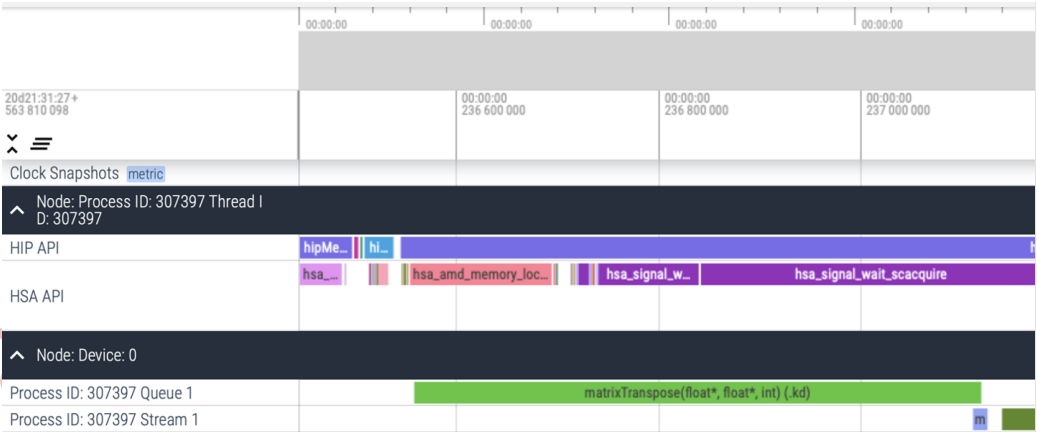
\includegraphics[width=1\linewidth]{FileAusiliari/Screenshots/Figure7-5.png}
    \caption{使用 Perfetto 視覺化 rocprofv2 捕捉的應用程式追蹤}
    \label{fig:captured application trace}
\end{figure}

\begin{lstlisting}[language=bash, caption={rocprofv2計數器的範例}, label={lst:rocprofv2 counter}]
gfx1030:0 : SQ_WAVES
: Count number of waves sent to SQs. {emulated, global, C1}
block SQ can only handle 8 counters at a time
\end{lstlisting}

這些條目可以理解如下:
\begin{enumerate}
    \item Gfx1030: GPU 架構
    \item 0: GPU ID. 目前的機器可能有多個 GPUs。
    \item SQ\_WAVES: 計數器名稱。通常,第一個底線之前是標記 GPU 區塊的名稱。在這裡,SQ 是個區塊,負責管理 wavefronts 和發出指令。
    \item Count number …: 計數器的描述
    \item Block SQ …: 使用效能計數器的硬體限制。每個 SQ 有 8 個計數器。因此我們在一次執行不能收集過多指標。
\end{enumerate}

要使用 rocprofv2 去收集硬體計數器和衍生的指標,可以使用 -i 選項提供輸入檔。

\begin{lstlisting}[language=bash, caption={使用rocprofv2分析kernel的命令}, label={lst:profile kernels with rocprofv2}]
rocprofv2 -i samples/input.txt <app_relative_path>
input.txt
\end{lstlisting}

輸入文件是個文字檔,提供 rocprofv2 進行計數器和指標的收集。它通常由四個部分組成,包含使用的效能計數器、分析的 GPUs、分析的 kernels 名稱和分析 kernels 的範圍。除了 pmc 欄位外,其他都是可選的。

\begin{lstlisting}[language=bash, caption={rocprofv2 kernel分析功能的輸入檔}, label={lst:Input file for kernel profiling feature of rocprofv2}]
pmc: SQ_WAVES TA_UTIL
range: 0:1
gpu: 0
kernel: matrixTranspose
\end{lstlisting}

輸入檔中的欄位描述如下:
\begin{itemize}
    \item PMC: 文字檔中以「pmc」開頭的列是使用者感興趣收集的指標群組。可以用 –list-counters 選項,查看產生的輸出,並從中選擇效能計數器。

    GPU 硬體資源限制一次執行分析可以收集的指標數量。如果收集過多指標,需要多次執行 kernels 來收集指標。在此情況下,輸入檔包含多列的 pmc。每個 pmc 列中的指標可以在每次執行 kernel 時進行收集。
    \item GPU: 關鍵字 gpu 開頭的列指定要收集硬體計數器的 GPU(s)。這能夠支援分析多個 GPUs,並且可以用逗號分隔指定多個 GPUs,例如:gpu: 1,3.
    \item Kernel: 關鍵字 kernel 開頭的列指定需要進行分析的 kernel 名稱。
    \item Range:  關鍵字 range 開頭的列指定 kernel 調度的範圍。指定範圍有助於在應用程式發生多個 kernel 調度時,使用者想要過濾某些 kernel 調度。在上面的例子,範圍 0:1 表示對一個 kernel 進行分析。
\end{itemize}

rocprofv2 命令列在輸出中,說明每個 kernel 中各個指標的一個值。在輸出格式方面,使用者仍然可以使用外掛程式去控制輸出格式。在這裡,我們將專注於檔案輸出和 Perfetto 的輸出。

檔案外掛程式替每個 kernel 產生新的資料條目(見以下範例)。每個 kernel 的基礎資訊(例如:gpu\_id、sgpr 計數等等)會在使用者指定的效能計數器前顯示。每個值都以「值的名稱(值)」的格式列出。

\begin{lstlisting}[language=bash, caption={rocprofv2 kernel 分析功能的輸出結果}, label={lst:Output of kernel profiling feature of rocprofv2}]
dispatch[1], gpu_id(0), queue_id(1), queue_index(0), pid(320661), tid
(320661), grd(1048576), wgr(16), lds(0), scr(0), arch_vgpr(8),
accum_vgpr(0), sgpr(128), wave_size(32), sig(140670227584384), obj(1)
, kernel-name("matrixTranspose"), start_time(1811083228321204),
end_time(1811083228892614)
, SQ_WAVES (65536.000000)
, GRBM_COUNT (288690.000000)
, GRBM_GUI_ACTIVE (288690.000000)
, SQ_INSTS_VALU (1048512.000000)
dispatch[2], gpu_id(0), queue_id(1), queue_index(2), pid(320661), tid
(320661), grd(1048576), wgr(16), lds(0), scr(0), arch_vgpr(8),
accum_vgpr(0), sgpr(128), wave_size(32), sig(140670227584384), obj(2)
, kernel-name("matrixTranspose"), start_time(1811083230510950),
end_time(1811083231072480)
, SQ_WAVES (65552.000000)
, GRBM_COUNT (286162.000000)
, GRBM_GUI_ACTIVE (286162.000000)
, SQ_INSTS_VALU (1048704.000000)
\end{lstlisting}

使用者也可以使用 Perfetto 外掛程式來產生可視化的輸出。以下是視覺化的 kernel 分析輸出的 Perfetto UI 截圖。最後一列是 kernel 執行時間軸,與在應用程式追蹤模式使用 –kernel-trace 是一樣的。其他上面的列表示使用者選擇的效能計數器。

這個視覺化圖表能夠清楚展示 kernel 執行時間的概況,以及效能指標在不同 kernels 中的變化情形。除此之外,使用者也可以藉由將滑鼠暫留或點擊某個條形圖,來取得效能指標的詳細值。

\subsection{ROCSys}

作為 rocprofv2 的一部分,ROCSys 是個命令列工具,可以在追蹤或分析應用程式時,控制效能分析的不同工作階段(啟動/開始/停止/離開)。當執行長時間的工作負載(DNN 訓練)時,使用者可能希望在應用程式執行時,控制應用程式並分析其中的部分。ROCSys 允許在執行期間開始/停止效能分析工作階段,並分析結果後退出工作階段。使用者可以從一個終端機(terminal)啟動工作階段,以及從另一個終端機(terminal)使用 ROCSys 來控制應用程式(開始/停止/離開)。

\begin{figure}
    \centering
    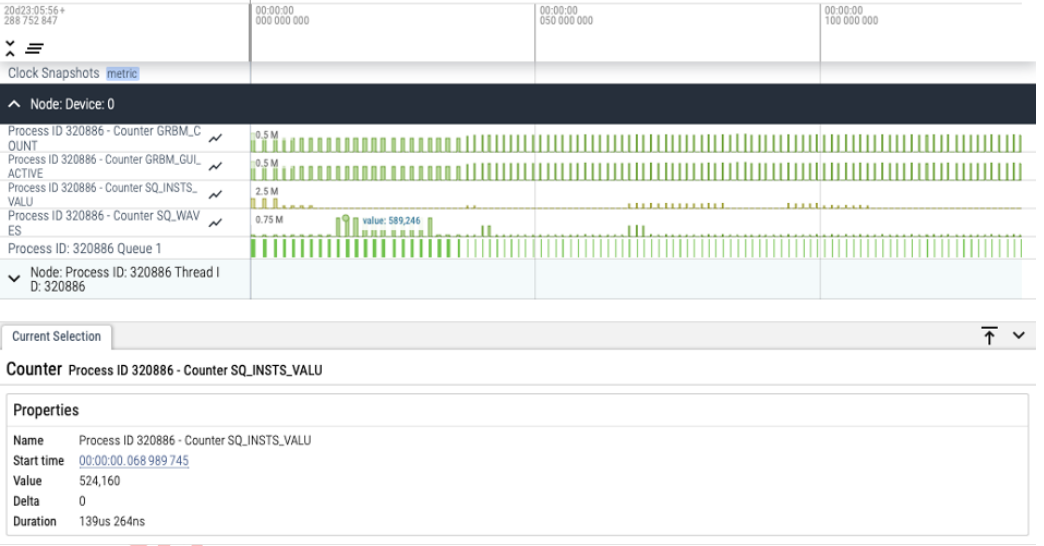
\includegraphics[width=1\linewidth]{FileAusiliari/Screenshots/Figure7-6.png}
    \caption{使用 Perfetto 視覺化 rocprofv2 捕捉的 kernel分析結果}
    \label{fig:captured kernel profiling results}
\end{figure}

我們接著展示使用 ROCSys 的整個流程。

首先,我們透過同時呼叫 ROCSys 和 rocprofv2 來建立一個工作階段。應用程式在 ROCSys 第二步工作階段啟動前將會暫停。

\begin{lstlisting}[language=bash, caption={使用 ROCSys 和 rocprofv2 建立工作階段}, label={lst:Creating a session using ROCSys and rocprofv2}]
/opt/rocm/bin/rocsys --session session1 launch rocprofv2 -i ../samples/
input.txt <long_running_app>
ROCSYS:: Session ID: 2109
ROCSYS Session Created!
ROCProfilerV2: Collecting the following counters:
- SQ_WAVES
- GRBM_COUNT
- GRBM_GUI_ACTIVE
- SQ_INSTS_VALU
- FETCH_SIZE
Enabling Counter Collection
\end{lstlisting}

第二步,在另一個終端機視窗,使用者可以啟動工具工作階段。啟動工作階段將觸發應用程式執行。

\begin{lstlisting}[language=bash, caption={開始分析工作階段}, label={lst:Starting the profiling session}]
/opt/rocm/bin/rocsys --session session1 start
ROCSYS:: Starting Tools Session...
Dispatch_ID(1), GPU_ID(1), ... // 一個 kernel 的所有指標
Dispatch_ID(2), GPU_ID(1), ... // 一個 kernel 的所有指標
Dispatch_ID(3), GPU_ID(1), ... // 一個 kernel 的所有指標
\end{lstlisting}

第三步,我們也可以暫停工具工作階段。暫停分析工作階段之後,應用程式將會繼續執行。當我們執行任何 rocsys 命令時,kernel 分析資訊將會轉到終端機上。這些 kernels 會執行在當前和過去之間的命令。

\begin{lstlisting}[language=bash, caption={停止分析工作階段}, label={lst:Stopping the profiling session}]
/opt/rocm/bin/rocsys --session session1 stop
ROCSYS:: Stopping Tools Session...
Dispatch_ID(22397), GPU_ID(1), ... // 一個 kernel 的所有指標
Dispatch_ID(22398), GPU_ID(1), ... // 一個 kernel 的所有指標
Dispatch_ID(22399), GPU_ID(1), ... // 一個 kernel 的所有指標
\end{lstlisting}

第四步,停止分析工作階段後,我們可以重新啟分析工作階段,分析結果和重新啟動工具工作階段。

\begin{lstlisting}[language=bash, caption={重啟分析工作階段}, label={lst:Restarting the profiling session}]
/opt/rocm/bin/rocsys --session session1 start
ROCSYS:: Starting Tools Session...
Dispatch_ID(22400), GPU_ID(1), ... // 一個 kernel 的所有指標
Dispatch_ID(22401), GPU_ID(1), ... // 一個 kernel 的所有指標
\end{lstlisting}

最後,我們離開工具工作階段。一旦離開工作階段,我們將不能再重啟它。

\begin{lstlisting}[language=bash, caption={離開分析工作階段}, label={lst:Exiting the profiling session}]
/opt/rocm/bin/rocsys --session session1 exit
Dispatch_ID(16828), GPU_ID(1), ... // 一個 kernel 的所有指標
Dispatch_ID(16829), GPU_ID(1), ... // 一個 kernel 的所有指標
ROCSYS:: Exiting Tools Session...Application might still be finishng up..
\end{lstlisting}

注意離開工作階段只有停止分析,應用程式仍然可能在背景執行/完成。假如不想再等待應用程式,可以使用 CTRL+C 離開應用程式或等待應用程式完成。

\section{使用 Hipify 移植 \term{CUDA} 程式到 \term{HIP}}

HIP 語言提供其中一項最有價值的工具是自動化的方法,能將整個用 \term{CUDA} 編寫的程式碼庫轉換成 \term{HIP}。有許多情況下,程式設計者或研究人員需要將 NVIDIA 系統開發的 \term{CUDA} 應用程式,移植並執行在 AMD GPU 上。可能是為了比較兩種不同平台上獲得的效能(其中一個學習 \term{HIP} 的重要動機,是避免鎖定在單一硬體供應商)。在 \term{HIP} 之前,只有手動將 \term{CUDA} 原始碼轉換成 \term{OpenCL} 的移植方式:一個繁瑣且容易出錯的路徑。有了 \term{ROCm},程式設計者現在可以利用簡單使用的原始碼對原始碼轉換器。除此之外,而且也許最重要的是,\term{HIP} 的使用能夠讓程式設計者/開發者使用他們現有的程式碼、技能和程式設計經驗,繼續用相同的投資來進行未來的開發。在本章中,我們詳細介紹這個過程並提供範例。我們也介紹一些常見轉換後的問題,以及用來解決這些問題的 Hipifying 工具。

\subsection{\term{Hipify}工具}

\term{ROCm} 提供兩種將 \term{CUDA} 轉換成 \term{HIP} 的工具,\term{Hipify-clang} 和 \term{Hipify-perl}。兩種都可以執行在 Linux 和 Windows 系統。每種方法都有其優點和缺點,這些會在本章後續討論。這些工具輸入 \term{CUDA} 原始檔,並且產生輸出 \term{HIP} 檔,包含 host-side APIs(例如:CUDA Driver、Runtime、Device 和 Runtime Compilation)。\term{Hipify}工具也可以轉換 cuComplex、cuBLAS、 cuDNN、cuFFT、cuRAND和cuSPARSE 函式庫 \cite{amd2021hip-supported-api}。
\\ \\ \bold{Hipify-clang}
\\ \term{Hipify-clang},顧名思義是一個基於 \term{clang},用來將 \term{CUDA} 程式碼轉換成 \term{HIP} 的工具。它的工作原理是將 \term{CUDA} 原始碼轉換成抽象的語法樹\cite{llvm2022abstract},接著透過轉換匹配器遍歷它。執行完整個過程後會產生 \term{HIP} 輸出。這個方法主要的優勢是使用 \term{clang} 前端。\term{Hipify-clang} 可以自動的支援任何新的 \term{CUDA} 版本,實現與新平台的互通性。此外,\term{Hipify-clang} 可以輕鬆解析並把複雜的結構轉換成 \term{HIP} 原始碼。這個轉換過程涵蓋聚集擴張、使用者命名空間中宣告的 \term{CUDA} 條目的重新定義、複雜的模板以及函式的參數列表。\term{Hipify-clang} 區分 device 和 host 函式呼叫,以及所需的標頭檔。然而,要確保輸入的 \term{CUDA} 程式碼是正確的;所有「includes」和「defines」也都要存在。錯誤的程式碼將不會被轉換,並且顯示錯誤。

\term{Hipify-clang} 需要取得相同 \term{clang} 編譯 \term{CUDA} 程式碼所需要的標頭才能處理檔案,因此需要安裝\term{CUDA},同時如果有多個安裝時,需要使用 「\bold{--cuda-path}」 選項。範例如下:

\begin{lstlisting}[language=bash]
./hipify-clang square.cu --cuda-path=/usr/local/cuda-11.6
\end{lstlisting}

先指定 Hipify-clang 的參數,再根據分割器,「\bold{\code{--}}」。假如需要編譯輸入檔案,再將參數傳遞給 \term{clang}。例如:

\begin{lstlisting}[language=bash]
./hipify-clang square.cu -- -std=c++17
\end{lstlisting}

基於 include 的檔案搜尋選項與 \term{clang} 及其他\term{C/C++} 編譯器中的選項相同:「\bold{-I=<directory>}」。使用 「\bold{-D=<macro>=<value>}」 選項,可以定義巨集(其值是可選的參數)。在這兩個選項中,可以省略 「\bold{=}」 符號,或是使用空格符號代替。命令列語法如下:

\begin{lstlisting}[language=bash]
./hipify-clang square.cu -I../../include -D USE_GPU -D=GFX=1033
\end{lstlisting}

有關編譯 \term{CUDA} 的更多資訊,請參考「Compiling CUDA with clang」手冊 \cite{amd2021compiling}。

\term{Hipify-clang} 支援編譯多個原始檔案,並且所有選項將用於每個檔案。

為了提供編譯選項給複雜的多個來源的 \term{CUDA} 專案做 Hipification,可以使用 \term{clang} 結合 \term{cmake} 產生 JavaScript 物件表示法(\term{JSON}, JavaScript Object Notation)的編譯資料庫。此資料庫可以使用 「\bold{-p=<folder with compile\_commands.json>}」 命令,來提供 \term{compile\_commands.json} 檔案。更多有關 \term{JSON} 編譯資料庫創建的資訊可以在 clang \term{JSON} 資料庫文件\cite{clang2018clang} 中找到。

某些 \term{CUDA} APIs 是以實驗性方式提供支援,預設不會進行轉換。如果要轉換它們,需要設置「\bold{--experimental}」選項。要查看所有支援和實驗性的 CUDA APIs,包含有關「appeared」、「deprecated」、「approved」版本的資訊,可以使用「\bold{./hipify-clang --md}」 或 「\bold{./hipify-clang --csv}」 命令,它們會分別以 markdown 或 CSV 的格式產生。這些檔案會被放到工作資料夾中。可以使用「\bold{--doc-format=<format>}」選項,設定要以完整、嚴格或緊湊的格式來產生 \term{CUDA2HIP} 文件。完整格式的文件範例列在 Table \ref{tab:CUDA2HIP},對應的 \term{CUDA} 和 \term{HIP} API 版本呈現在「A」、「D」、「R」和「E」行。「A」表示該 API 新增的版本、「D」 表示已經棄用、「R」 表示已經移除,而「E」表示 API 成為實驗性 \term{HIP} 的發布版本(通常是\term{HIP}最新發布的版本)。如果 \term{HIP} API 不存在,表示對應的 \term{CUDA} API 尚未在 \term{HIP} 中支援。

\begin{table}[htbp]
    \centering
    \begin{tabular}{@{}lccclcccc}
        \toprule
        \multicolumn{1}{c}{CUDA} & \multicolumn{1}{c}{A} & \multicolumn{1}{c}{D} & \multicolumn{1}{c}{R} & \multicolumn{1}{c}{HIP} & \multicolumn{1}{c}{A} & \multicolumn{1}{c}{D} & \multicolumn{1}{c}{R} & \multicolumn{1}{c}{E} \\
        \midrule
        cudaDeviceSetGraphMemAttribute & 11.4 \\
        cudaGraphAddChildGraphNode & 10.0 \\
        cudaGraphAddDependencies & 10.0 &&& hipGraphAddDependencies & 4.5.0 &&& 4.5.0 \\
        cudaGraphAddEmptyNode & 10.0 &&& hipGraphAddEmptyNode & 4.5.0 &&& 4.5.0 \\
        \bottomrule
    \end{tabular}
    \caption{完整格式下 CUDA2HIP 的文件範例}
    \label{tab:CUDA2HIP}
\end{table}

\term{Hipify-clang} 在預處理器的行為上,與一般的 \term{clang} 及其他 \term{C/C++} 編譯器有一個重要的差異,這個差異與解析條件式的預處理器區塊 \#if、\#else 和 \#endif 有關。大多編譯器在計算編譯條件時,會跳過 false 的條件區塊,然而在轉換成 \term{HIP} 時,\term{Hipify-clang} 預設不會跳過 false 的條件區塊。此行為也許會使編譯錯誤,與需要依賴平台才能執行的程式碼一樣。如果要改變 \term{Hipify-clang} 預處理器的預設,應該指定「\bold{--skipexcluded-preprocessor-conditional-blocks}」選項。

\term{HIP} 目前支援 \term{CUDA} kernel 啟動語法 \cite{nvidia2022cuda} 及其 kernel 執行配置。然而,為了提升相容性,\term{Hipify-clang} 轉換這種語法,將其變成一般的函式呼叫。以下是個 \term{CUDA} kernel 啟動語法和轉換成 \term{hipLaunchKernelGGL} 的範例。

\begin{lstlisting}[language=bash]
matrixTranspose<<<dimGrid, dimBlock>>>(
    gpuTransposeMatrix, gpuMatrix, WIDTH);
hipLaunchKernelGGL(
    matrixTranspose, dim3(dimGrid), dim3(dimBlock),
    0, 0, gpuTransposeMatrix, gpuMatrix, WIDTH);
\end{lstlisting}

如果要在 \term{Hipify} 的程式碼中保留 \term{CUDA} kernel 的啟動語法,要使用「\bold{--cudakernel-execution-syntax}」選項。在未來的 \term{Hipify} 版本中,預設將會有此選項,並且 kernel 呼叫將會與 CUDA 語法類似。

「\bold{--inplace}」選項讓 \term{Hipify-clang} 可以直接修改輸入檔,將輸入的 \term{CUDA} 檔案直接替換成 \term{HIP} 檔案。這對於移植大型多源專案時非常有幫助,因為最佳作法是先複製整個程式碼庫再將其 Hipify。之後,使用者則可以根據需求進行目錄比較。

\term{Hipify-clang} 會從不同角度收集已轉換及未轉換的 APIs 統計資料。要輸出這些統計資料到標準輸出,應該加入 「\bold{--print-stats}」 選項。如果要以 CSV 檔的格式,應該使用「\bold{--print-stats-csv}」選項。範例統計資料會在本章後續部分展示,並進行範例解析說明。對於多個原始檔的情況,則會提供個別文件和整體的統計資料,此功能在分析已進行 Hipified 的大型 \term{CUDA} 專案時非常有幫助。舉例來說,所有未轉換的 APIs 會顯示在同個地方,並且每個實例都會被計算。

另一個實用的工具是「\bold{--examine}」,它提供類似於「\bold{--print-stats}」的命令來產生統計資料;不過,它不會產生 Hipified 的檔案,因此可以更快地評估可移植性。

「\bold{--o-dir}」選項允許程式設計者指定 Hipified 統計資料的輸出目錄。

如果要查看所有可用的選項及其描述,我們可以使用「\term{--help}」選項。

以下為在使用 \term{Hipify-clang} 進行 Hipification 時,最常見產生錯誤與警告的列表。

\begin{itemize}
    \item 不支援的 API。這個警告代表 \term{HIP} 尚未支援此 API。如果可以,應該重寫原始碼,避免使用不支援的 API。如果程式設計者認為此 API 不可缺少,而且在沒有它的情況下,應用程式便無法執行,可以在此處提出問題 \cite{amd2021hip}。此類警告的範例如下:

    \begin{lstlisting}[language=bash]
    intro.cu.hip:77:3: warning: CUDA identifier is unsupported in HIP.
      CUmemLocation memLoc.
      ^
    \end{lstlisting}
    
    \item 實驗性的 API。該警告表示 API 只是實驗性,而且並不能保證正確。如果要使用實驗性的 APIs Hipification,可以使用 「\bold{--experimental}」選項。以下我們看一下這類警告的範例:
    
    \begin{lstlisting}[language=bash]
    Simplemechs.cu.hip:35:1: warning: CUDA identifier is experimental
    in HIP. To Hipify it, use the '--experimental' option.
    \end{lstlisting}
    
    \item 已棄用的 API。該警告表示 API 在 \term{CUDA} 已經棄用,但在 \term{HIP} 仍然支援並啟用。
    
    \begin{lstlisting}[language=bash]
    intro.cu.hip:46:3: warning: 'cudaThreadSynchronize' is deprecated
    [-Wdeprecated-declarations]
      cudaThreadSynchronize().
      ^
    \end{lstlisting}
    
    \item 已移除的 API。該錯誤訊息代表 API 從 \term{CUDA} 刪除了。在這種情況下,原始碼要重寫成沒有已移除的 API;否則,要對那個 API 還存在的 \term{CUDA} 版本執行 Hipification:
    
    \begin{lstlisting}[language=bash]
    intro.cu.hip:78:12: error: use of undeclared identifier
    'CU_COMPUTEMODE_EXCLUSIVE'
      if (cm == CU_COMPUTEMODE_EXCLUSIVE).
                ^
    \end{lstlisting}


\end{itemize}

假如編譯錯誤發生後,Hipified 的輸出將不會產生,或產生不正確。因此,產生的統計資料將也會不正確:

\begin{lstlisting}[language=bash]
ERROR: Statistics is invalid due to failed hipification.
\end{lstlisting} 
\bold{Hipify-perl}
\\ \term{Hipify-perl} 是基於 \term{Perl} 自動產生,大量使用正規語言表示式的腳本。要產生 \term{Hipify-perl},執行「\bold{./hipify-clang --perl}」,\term{Hipify-perl} 將會自動產生,並且在預設的工作目錄。可以用「\bold{--o-hipifyperl-dir}」選項指定產生 \term{Hipify-perl} 檔案的輸出目錄。

不同於 \term{Hipify-clang} 的是,\term{Hipify-perl} 不需要安裝 \term{CUDA},而且不需要依靠第三方工具。只需要 \term{Perl},而且原始檔不必在語法上正確。然而,當依靠正規語言表示式,一些 \term{CUDA} 程式碼有可能不能轉換成 \term{HIP}。此工具現在還不能擴展到所有巨集、區分在使用者命名空間中宣告的 \term{CUDA} 條目的重新定義、應用使用者命名空間、為 API 或資料型別加入新的指令、區分 device/host 函式呼叫、注入標頭檔或解析複雜的函式參數列表。

通常,\term{Hipify-perl} 工作效率較高,但比 \term{Hipify-clang} 慢。在大多數的情況下,程式設計者可以透過手動更正錯誤和警告,來改善轉換相關的問題。

這個基於腳本的轉換器的目標是提供了一個快速的工具,用於臨時 Hipification 任何的 \term{CUDA} 程式碼,並估計移值所需的工作量。要移值有大量原始檔的複雜專案時,建議使用 \term{Hipify-clang}。

\term{Hipify-perl} 也支援多輸入原始檔,並且提供與 Hipify-clang 相同含意的以下選項:

\begin{lstlisting}[language=bash]
-examine, -experimental, -inplace, -o=, -print-stats
\end{lstlisting}

與 \term{Hipify-clang} 不同的是,\term{Hipify-perl} 支援一些特定選項,以滿足 \term{Hipify-perl} 所需的腳本功能。

「\bold{-whitelist=<list>}」選項讓使用者指定一個以逗號分隔的標示符清單,這些標示符將不會進行 hipified 轉換;否則,某些 APIs 可能錯誤地轉換。

「\bold{-quiet-warnings}」會停止所有警告。「\bold{-excludedirs=}」和「\bold{-exclude-files=}」排除指定的目錄或檔案,這在處理多個來源檔 Hipification 時非常有幫助。

\subsection{一般的 Hipify 指南}

鼓勵程式設計者在 Hipifying \term{CUDA} 時,遵循下列基本原則:
\begin{itemize}
    \item 在單獨原始碼的目錄執行 Hipify,以便產生單獨的原始程式碼樹。這樣可以輕鬆地比較兩個目錄中的原始程式碼。此方法允許使用者輕鬆的區分不同的版本,並在目標平台使用他們所需的版本。
    \item 在成功 Hipification 後,執行編譯產生的 \term{HIP} 程式碼,並驗證結果是否與原始 \term{CUDA} 或 CPU 版本相符,且效能表現良好。然而,這並不是每次都可行。舉例來說,應用程式依靠隨機數字產生器或隨機應用(例如:機器學習),即使在同一平台多次執行,也可能不會每次都得到相同結果。在比較執行結果時,正確性是首先要考量,接下來才是準確度和效能。
    \item 程式設計者應該在進行 Hipification 前,先對應用程式及原始碼有基礎的了解,這樣才更容易識別並修正編譯錯誤,同時也能更有效地解決執行時的問題。
    \item 程式設計者應該查閱最新的 \term{HIP} 手冊\cite{amd2021hip-supported-api},確認在 \term{CUDA} 中所使用的 API 呼叫是否支援。
\end{itemize}

\subsection{矩陣轉置 Hip 化}

在本節中,我們使用簡單的 \term{CUDA} 範例研究 Hipification 的過程,MatrixTranspose.cu,如 \lstref{lst:CUDA matrix-transpose example snippet} 所示,並使用 \term{Hipify-clang} 工具將其轉換成 \term{HIP}。

\begin{lstlisting}[language=C++, caption={CUDA 矩陣轉置的範例片段}, label={lst:CUDA matrix-transpose example snippet}]
cudaDeviceProp devProp;
CHECK(cudaGetDeviceProperties(&devProp, 0));
// 在 GPU 上記憶體分配
CHECK(cudaMalloc((void**)&gpuMatrix, NUM * sizeof(float)));
CHECK(cudaMalloc((void**)&gpuTransposeMatrix, NUM * sizeof(float)));
// 記憶體從 CPU 傳輸到 GPU
CHECK(cudaMemcpy(gpuMatrix, Matrix, NUM * sizeof(float), cudaMemcpyHostToDevice));
const uint32_t THREADS_PER_BLOCK_X = 4;
const uint32_t THREADS_PER_BLOCK_Y = 4;
const uint32_t THREADS_PER_BLOCK_Z = 1;
const uint32_t GRID_X = uint32_t(WIDTH / THREADS_PER_BLOCK_X);
const uint32_t GRID_Y = uint32_t(WIDTH / THREADS_PER_BLOCK_Y);
dim3 dimGrid(GRID_X, GRID_Y);
dim3 dimBlock(THREADS_PER_BLOCK_X, THREADS_PER_BLOCK_Y, THREADS_PER_BLOCK_Z);
// Kernel 啟動
matrixTranspose<<<dimGrid, dimBlock>>>(gpuTransposeMatrix, gpuMatrix, WIDTH);
// 記憶體從 device 傳輸到 host
CHECK(cudaMemcpy(TransposeMatrix, gpuTransposeMatrix, NUM * sizeof(float), cudaMemcpyDeviceToHost));
for (uint32_t i = 0; i < NUM; ++i){
  printf("Matrix[%d]: %.2f  | cpuTransposeMatrix[%d]: %.2f\n", i, Matrix[i], i, cpuTransposeMatrix[i]);
}
\end{lstlisting}

要展示 hipifying CUDA 程式碼的實用性,在範例中使用 matrixTransposeGPU 函式。我們 Hipify 是基於 CUDA 11.6 版本的程式碼,並產生對應的統計資料。完整的應用程式程式碼會在本文附帶的原始碼中提供。要 Hipify 檔案 MatrixTranspose.cu,我們使用以下命令:

\begin{lstlisting}
./hipify-clang MatrixTranspose.cu --print-stats --print-stats-csv
--cuda-kernel-execution-syntax
--cuda-path=/usr/local/cuda-11.6
\end{lstlisting}

執行這個命令產生一個矩陣轉置操作的 \term{HIP} 版本,產生 MatrixTranspose.cu.hip 檔案,如\lstref{lst:Hipified matrix-transpose example snippet}所示。

\begin{lstlisting}[language=C++, caption={Hipified 矩陣轉置的範例片段}, label={lst:Hipified matrix-transpose example snippet}]
hipDeviceProp_t devProp;
CHECK(hipGetDeviceProperties(&devProp, 0));
// 在 GPU 上記憶體分配
CHECK(hipMalloc((void**)&gpuMatrix, NUM * sizeof(float)));
CHECK(hipMalloc((void**)&gpuTransposeMatrix, NUM * sizeof(float)));
// 記憶體從 CPU 傳輸到 GPU
CHECK(hipMemcpy(gpuMatrix, Matrix, NUM * sizeof(float), hipMemcpyHostToDevice));
const uint32_t THREADS_PER_BLOCK_X = 4;
const uint32_t THREADS_PER_BLOCK_Y = 4;
const uint32_t THREADS_PER_BLOCK_Z = 1;
const uint32)t GRID_X = uint32_t(WIDTH / THREADS_PER_BLOCK_X);
const uint32_t GRID_Y = uint32_t(WIDTH / THREADS_PER_BLOCK_Y);
dim3 dimGrid(GRID_X, GRID_Y);
dim3 dimBlock(THREADS_PER_BLOCK_X, THREADS_PER_BLOCK_Y, THREADS_PER_BLOCK_Z);
// Kernel 啟動
matrixTranspose<<<dimGrid, dimBlock>>>(gpuTransposeMatrix, gpuMatrix, WIDTH);
// 記憶體從 GPU 傳輸到 CPU
CHECK(hipMemcpy(TransposeMatrix, gpuTransposeMatrix, NUM * sizeof(float), hipMemcpyDeviceToHost));
\end{lstlisting}

\lstref{lst:Matrix-transpose HIP conversion statistics} 顯示轉換統計資料,輸出到 \term{stdout} 以便檢查,並報告了成功移植的原始程式碼百分比。列表也有 \term{CUDA} 轉換成 \term{HIP} API 呼叫的資訊。我們可以看到所有的 APIs 都被轉換,CONVERSION 為 100\% 證實它。總共 13 個 CUDA APIs 被轉換成 HIP。我們還可以看到三種已轉換 APIs 的類型 (即 error、 device 和 memory)僅來自\term{CUDA Runtime} API。\lstref{lst:Matrix-transpose HIP conversion statistics} 的最後一部分說明了各種成功轉換的 \term{CUDA} API 類型的數量。

\begin{lstlisting}[language=bash, caption={矩陣轉置的 HIP 轉換統計資料}, label={lst:Matrix-transpose HIP conversion statistics}]
[HIPIFY] info: file 'MatrixTranspose.cu' statistics:
  CONVERTED refs count: 13
  UNCONVERTED refs count: 0
  CONVERSION %: 100.0
  REPLACED bytes: 182
  TOTAL bytes: 3383
  CHANGED lines of code: 11
  TOTAL lines of code: 78
  CODE CHANGED (in bytes) %: 5.4
  CODE CHANGED (in lines) %: 14.1
  TIME ELAPSED s: 0.75
[HIPIFY] info: CONVERTED refs by type:
  error: 1
  device: 1
  memory: 6
  include_cuda_main_header: 1
  type: 1
  numeric_literal: 3
[HIPIFY] info: CONVERTED refs by API:
  CUDA RT API: 13
[HIPIFY] info: CONVERTED refs by names:
  cudaDeviceProp: 1
  cudaFree: 2
  cudaGetDeviceProperties: 1
  cudaGetErrorString: 1
  cudaMalloc: 2
  cudaMemcpy: 2
  cudaMemcpyDeviceToHost: 1
  cudaMemcpyHostToDevice: 1
  cudaSuccess: 1
  cuda_runtime.h: 1
\end{lstlisting}

我們現在已經使用 \term{HIP} 編譯器編譯應用程式,並執行它在 AMD GPU 上。要執行程式碼,請使用下列命令:

\begin{lstlisting}
hipcc MatrixTranspose.cu.hip -o MatrixTranspose -v
\end{lstlisting}

選項 「\bold{v}」 指定要詳細的編譯器輸出。

我們接下來將透過在 AMD GPU 平台編譯並執行我們 Hipified 的程式碼,來展示 \term{HIP} 的可移植性。注意環境變數 \term{HIP\_PLATFORM} 應該設定為 \bold{nvidia}:

\begin{lstlisting}
export HIP_PLATFORM=nvidia
\end{lstlisting}

對於編譯,我們加上「\term{-x cu}」 選項。

\begin{lstlisting}
hipcc MatrixTranspose.cu.hip -o MatrixTranspose -x cu -v
\end{lstlisting}

假如設定有兩個 GPUs,例如一個啟用 NVIDIA 的 GPU,一個啟用 ROCm 的 GPU,則兩個編譯的可執行檔應該都能成功執行。

\subsection{常見的陷阱及解決方案}

Hipifying \term{CUDA} 原始程式碼時需要注意以下幾點:

\begin{itemize}
    \item  Hipify 工具可以成功轉換受支援的 \term{CUDA} API 函式呼叫和資料型別。然而,在撰寫本書時,\term{HIP}並不支援所有的\term{CUDA}函式。有些APIs只有實驗性支援,有些則完全不支援。若想了解請查詢列表,參考\cite{amd2021hip-supported-api}。
    \item 在 kernel 的功能方面,最近 \term{CUDA} 引入 warp-level shuffle sync,但現在 \term{HIP} 並不支援。程式設計者必須小心檢查這些函式,並用\term{HIP}支援的 warp shuffle 版本替換掉它們。
    \item 許多 \term{CUDA} 程式碼庫依靠使用 \term{warp\_id} 計算偏移量和操作。在 \term{CUDA} 設備中,wavefront 大小是 32。然而,在 AMD GPUs(non-RDNA) 上,wavefront 大小是 64。因此,任何依靠 wavefront 為 32 才會正確的程式碼執行時必須手動更新。在 \term{CUDA} kernel 程式碼中,使用 \term{warpSize} 變數,而不是將 \term{warpSize} 設成固定的常數值 32。當轉換成 \term{HIP} 時,\term{warpSize} 變數會自動轉換成正確的 wavefront 值。
    \item 一些 NVIDIA GPU 專用的 APIs 無法移植到 AMD GPU,並且可能永遠沒辦法。好的一面是,這類例子很少,不需要過度擔心。
\end{itemize}

\section{結論}

在本章中,我們研究了 \term{ROCm} 提供的重要工具。首先,我們討論 \term{ROCmInfo},這個工具可以用來獲得有關 ROCm 堆疊(stack)和系統硬體設定的詳細資訊。第二個工具是 \term{ROCm SMI},它提供簡單的命令列工具去控制 GPU kernel、記憶體時脈、功率管理、溫度和使用率。程式設計者可以將 \term{SMI} 函式直接嵌入應用程式中。\term{ROCm} 也提供簡單使用的 \term{ROCm-SMI-Lib} 函式。我們也介紹 \term{ROCm} 除錯器 \term{rocgdb}。它允許程式設計者除錯時逐行偵錯 GPU kernel。我們還介紹了 \term{rocTracer},它可以提供應用程式效能的測量資料,並展示如何使用 \term{rocProf},透過 GPU 的硬體效能計數器,來取得詳細的效能分析資料。該資料對調適 GPU 效能至關重要。在本書後面,我們使用這工具做額外的效能分析。最後,我們介紹如何使用 ROCm 提供的 Hipify 將 CUDA 程式碼轉換成 HIP。我們也討論將 CUDA 程式碼移植成 HIP 時,一般常見的陷阱和解法。程式設計者應該經常檢查 ROCm 最新版的文件,以了解哪些 APIs 和功能是被支援的,這樣可以讓移植過程更不容易出錯。AMD 持續與研究機構合作,形成了豐富的新開源效能分析與除錯工具生態系統,例如效能 API (\term{PAPI}, the Performane API)、調適和分析實用工具 (\term{TAU}, the Tuning and Analyses Utility)以及勞倫斯利佛摩國家實驗室(LLNL, the Lawrence Livermore National Laboratory)高效能計算(HPC, high-performance computing)工具組(\term{HPCToolkit}),僅舉幾個例子。這些工具將在稍後的章節中討論。